\documentclass[a4paper,14pt]{article} % тип документа
%\documentclass[14pt]{extreport}
\usepackage{extsizes} % Возможность сделать 14-й шрифт


\usepackage{geometry} % Простой способ задавать поля
\geometry{top=25mm}
\geometry{bottom=35mm}
\geometry{left=20mm}
\geometry{right=20mm}
%%%Библиотеки
	%\usepackage[warn]{mathtext}	
	\usepackage[T2A]{fontenc} % кодировка
	\usepackage[utf8]{inputenc} % кодировка исходного текста
	\usepackage[english,russian]{babel} % локализация и переносы
	\usepackage{caption}
	\usepackage{listings}
	\usepackage{amsmath,amsfonts,amssymb,amsthm,mathtools}
	\usepackage{wasysym}
	\usepackage{graphicx}%Вставка картинок правильная
	\usepackage{float}%"Плавающие" картинки
	\usepackage{wrapfig}%Обтекание фигур (таблиц, картинок и прочего)
	\usepackage{fancyhdr} %загрузим пакет
	\usepackage{lscape}
	\usepackage{xcolor}
	\usepackage[normalem]{ulem}
	\usepackage{hyperref}

%%%Конец библиотек




%%%Настройка ссылок
	\hypersetup
	{
		colorlinks=true,
		linkcolor=blue,
		filecolor=magenta,
		urlcolor=blue
	}
%%%Конец настройки ссылок


%%%Настройка колонтитулы
	\pagestyle{fancy}
	\fancyhead{}
	\fancyhead[L]{Вопрос по выбору}
	\fancyhead[R]{Талашкевич Даниил, группа Б01-009}
	\fancyfoot[C]{\thepage}
%%%конец настройки колонтитулы



							\begin{document}
						%%%%Начало документа%%%%


%%%Начало титульника
\begin{titlepage}

	\newpage
	\begin{center}
		\normalsize Московский физико-технический институт \\(госудраственный 			университет)
	\end{center}

	\vspace{6em}

	\begin{center}
		\Large Устный экзамен по физике \\(электричество и магнетизм) \\
        \Large Вопрос по выбору
	\end{center}

	\vspace{1em}

	\begin{center}
		\Large \textbf{Ферромагнетизм}
	\end{center}

	\vspace{2em}

	\begin{center}
		\large Талашкевич Даниил Александрович\\
		Группа Б01-009
	\end{center}

	\vspace{\fill}

	\begin{center}
	Долгопрудный \\2021
	\end{center}
	
\end{titlepage}
%%%Конец Титульника



%%%Настройка оглавления и нумерации страниц
	\thispagestyle{empty}
	\newpage
	\tableofcontents
	\newpage
	\setcounter{page}{1}
%%%Настройка оглавления и нумерации страниц


					%%%%%%Начало работы с текстом%%%%%%
				
\section{Ферромагнетизм}

Ферромагнетиками называют твердые тела, которые могут обладать спонтанной намагниченностью, т.е. намагничены уже в отсутствии магнитного поля. Типичными представителями ферромагнетиков являются металлы: железо, кобальт, никель. Ферромагнетики способны сильно намагничиваться даже в небольших полях.

Существенным отличием ферромагнетиков от диа- и парамагнетиков является наличие у ферромагнетиков самопроизвольной (спонтанной) намагниченности в отсутствие внешнего магнитного поля. Наличие у ферромагнетиков самопроизвольного магнитного момента в отсутствие внешнего магнитного поля означает, что электронные спины и магнитные моменты атомных носителей магнетизма ориентированы в веществе упорядоченным образом.

Характерной особенностью ферромагнетиков является сложная нелинейная зависимость между $\overrightarrow{I}$ и $\overrightarrow{H}$. По мере возрастания $\overrightarrow{H}$ намагниченность $\overrightarrow{I}$ сначала быстро растет, а затем становится практически постоянной: $\overrightarrow{I} = \overrightarrow{I_S}$ (насыщение), т.е. кривая $I = I(H)$ переходит в горизонтальную прямую. Магнитная индукция $\overrightarrow{B} = \overrightarrow{H} + 4\pi\overrightarrow{I}$ также растет с возрастанием поля $\overrightarrow{H}$, а в состоянии насыщения $\overrightarrow{B} = \overrightarrow{H} + 4\pi\overrightarrow{I_S}$.

Ввиду нелинейной связи между $\overrightarrow{I} = \chi\overrightarrow{H}$ и $\overrightarrow{H}$ для ферромагнетиков магнитная восприимчивость $\chi$ и магнитная проницаемость $\mu = 1 + 4\pi\chi$ могут иметь тензорнный характер(вектора $\overrightarrow{I}$ и $\overrightarrow{H}$ не сонаправлены). Эти функции рассматриваются как функции напряженности поля $\overrightarrow{H}$.

Участок 1 - область обратимого намагничивания, где $M=\chi H$. В этой области происходят процессы упругого смещения границ доменов: увеличивается размер тех доменов, магнитный момент которых близок к направлению магнитного поля, и уменьшаются размеры доменов с противоположным направлением магнитного момента.

Участок 2 характеризуется квадратичной зависимостью $M$ от $H .$ В этой области также идёт процесс обратимого смещения границ, но проявляется нелинейный характер зависимости намагниченности от поля.

Область максимальной скорости роста намагниченности 3 соответствует необратимым смещениям стенок между доменами («стенок Блоха»): им приходится преодолевать «препятствия» в виде примесей, дислокаций и дефектов кристаллической решётки. Когда стенка наталкивается на такое препятствие, она останавливается и держится, пока поле не достигнет порогового значения, при котором она внезапно срывается. Таким образом, движение доменной стенки приобретает скачкообразный характер («скачки Баркгаузена»).

В достаточно сильных полях движение стенок прекращается, и энергетически выгодным становится поворот магнитных моментов тех оставшихся доменов, у которых магнитный момент не совпадает с направлением поля (область 4).

И, наконец, при некотором значении поля (участок 5) все магнитные моменты выстраиваются по полю - намагниченность образца достигает насыщения $\left(M=M_{s}\right)$.

\begin{figure}[H]
	\center{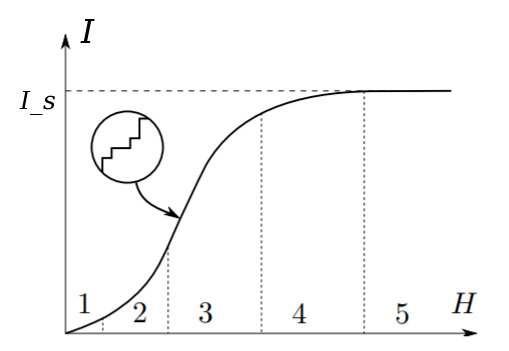
\includegraphics[scale = 0.5]{pic_1.png}}
	\caption{Начальная кривая намагничивания ферромагнетика}
\end{figure}

Вторая характерная особенность ферромагнетиков состоит в том, что для них зависимость $\overrightarrow{I}$ от $\overrightarrow{H}$ не однозначна, а определяется предшествующей историей намагничивания ферромагнитного образца. Это явление называется \textbf{магнитным гистерезисом}. Благодаря гистерезису намагничивание и перемагничивание ферромагнетиков сопровождается выделением тепла, называемого теплом гистерезиса.

\begin{figure}[H]
	\center{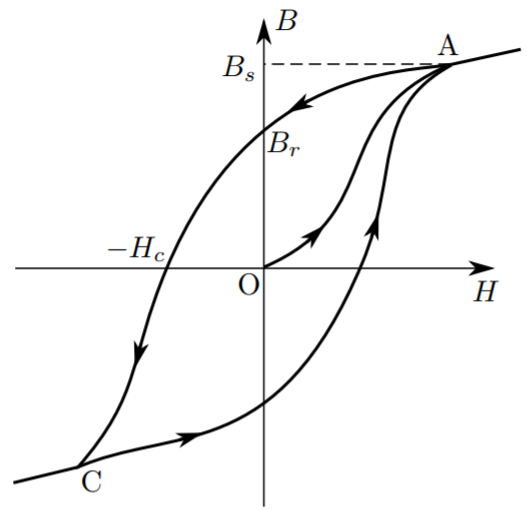
\includegraphics[scale = 0.5]{pic_2.png}}
	\caption{Начальная кривая намагничивания (OA) и предельная петля гистерезиса}
\end{figure}

Третья характерная особенность ферромагнетиков, состоит в том, что для любого ферромагнетика существует определенная температура $T = T_K$ называемая температурой или точкой Кюри, при переходе через которую вещество ферромагнетика претерпевает фазовый переход второго рода. Вещество является ферромагнетиком только при $T < T_K$. При $T > T_K$ вещество становиться парамагнетиком. Магнитная восприимчивость подчиняется закону Кюри-Вейсса 
\[\chi = \frac{Const}{T - T_K}\]

\section{Теория ферромагнетизма Вейсса}

В теории Вейсса силы взаимодействия между атомами формально сводятся к "эффективному"\ полю, которое и ориентирует атомы ферромагнетика. Эффективное поле складывается из обычного макроскопического поля в веществе $\overrightarrow{H}$ и некоторого гипотетического "молекулярного поля". Согласно предположению Вейсса:

\[\overrightarrow{B_\text{эфф}} = \overrightarrow{H} + b\overrightarrow{I}\]

где $b$ -- некоторая положительная постоянная, характеризующая свойства различных ферромагнетиков. Она называется постоянной Вейсса.

Исходя из этих предположений, рассчитаем намагничивание ферромагнетика $I$. Для этого заменим в теории Ланжевена поле $\overrightarrow{H}$ на эффективное поле $B_\text{эфф}$.

Воспользуемся распределением Больцмана. Число атомов в единице объема ферромагнетика, угол оси которых с направлением эффективного поля $B_\text{эфф}$ лежит в пределах $\theta$ и $\theta +d\theta$, будет равно 

\[dn = C e^{x\cos{\theta}}\sin{\theta d\theta}\]

\[x = \frac{\mathfrak{M}B_\text{эфф}}{kT} = \frac{\mathfrak{M}(H + bI)}{kT}\]

Определим константу C из условия того, что общее число всех атомов должно равняться n:

\[n = \int{dn} = C\int\limits_{0}^{\pi}{e^{x\cos{\theta}}\sin{\theta d\theta}} = \frac{C}{x}(e^x - e^{-x})\]

Получаем выражение для C:

\[C = \frac{xn}{e^x-e^{-x}}\]

Теперь определим результирующий магнитный момент единицы объема $I$. Вектор $I$ считаем параллельным эффективному полю $B_\text{эфф}$. Общий момент $dn$ атомов, оси которых лежат между $\theta$ и $\theta + d\theta$, равен $\mathfrak{M}dn$. Проекция этого момента на направление $B_\text{эфф}$ равна $\mathfrak{M}dn\cos{\theta}$. Отсюда получаем:

\[I = \int{\mathfrak{M}\cos{\theta}dn} = C\mathfrak{M}\int{e^{x\cos{\theta}}\cos{\theta}\sin{\theta} d\theta} = C\mathfrak{M}\left(\frac{e^x + e^{-x}}{x} - \frac{e^x-e^{-x}}{x^2}\right)\]

\[I = n\mathfrak{M}\left(\coth{x} - \frac{1}{x}\right) = n\mathfrak{M}L(x)\]

$L(x)$ -- функция Ланжевена.\\
Заметим, что $I_S = n\mathfrak{M}$, тогда выразим $I$ из предыдущих уравнений:
\[I = I_S L(x), ~I = \frac{kTn}{I_S b}x - \frac{H}{b}\]

Исследуем эту систему графически. Будем откладывать по горизонтальной оси величину x, а по вертикальной -- намагничивание I.

\begin{figure}[H]
	\center{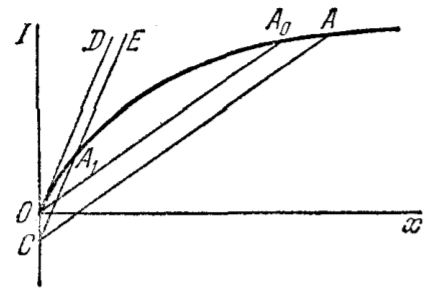
\includegraphics[scale = 0.8]{pic_3.png}}
	\caption{Зависимость I(x)}
\end{figure}

Допустим сначала, что наклон прямой CA меньше наклона кривой
\[\frac{kTn}{I_Sb} < I_S\left(\frac{dL}{dx}\right)_{x=0}\]
\[T < \frac{I_S^2 b}{kn}\left(\frac{dL}{dx}\right)_{x=0} = T_K\]
Прямая пересечет прямую Ланжевена в точке A, оридината и будет намагничиванием ферромагнетика I.

Если уменьшать поле H до нуля точка C будет подниматься к точке O, а точка A -- перемещаться к точке $A_0$. Когда поле H обратиться в нуль, ферромагнетик останется намагниченным -- его намагничивание представится ординатой точки $A_0$. 

Стоит отметить, что ферромагнетик будет спонтанно намагничен и в том случае, когда он вообще не вносился ни в какое магнитное поле, потому что благодаря гипотетическому взаимодействию между атомами, введенному Вейсом, состояние спонтанного намагничивания "энергетически выгодно".

Таким образом, при $T < T_K$ ферромагнетик должен быть спонтанно намагничен. Энергии теплового движения недостаточно, чтобы разрушить это намагничивание. Величина $T_K$ называется температурой или точкой Кюри.

Ниже точки Кюри из-за наличия спонтанного намагничивания $\chi$ и $\mu$ являются функциями от H:
\[\chi = \frac{dI}{dH},~ \mu = \frac{dB}{dH}\]

Теперь предположим, что наклон прямой CA больше наклона кривой Ланжевена в точке O. Это означает, что $T > T_K$. Тогда при отсутствии магнитного поля прямая CA займет положение OD, т.е. пересечет функцию Лагжевена только в начале координат. При этом спонтанное намагничивание не возникнет: намагничивание разрушается тепловым движением. Поэтому, чтобы намагнитить необходимо приложить магнитное поле. Прямая CA займет положение CE и пересечет кривую Ланжевена в точке $A_1$. Из эксперементов известно, что ордината $OC = -\frac{H}{b}$ мала, а поэтому мал и учаток $OA_1$ кривой Ланжевена.

\[L(x) = \left(\frac{dL}{dx}\right)_{x=0}x\]

\[I = I_S L(x) = I_S \left(\frac{dL}{dx}\right)_{x=0}x\]

\[T_K = \frac{I_S^2 b}{kn}\left(\frac{dL}{dx}\right)_{x=0} \Rightarrow \left(\frac{dL}{dx}\right)_{x=0} = \frac{T_K k n}{I_S^2b}\]

\[I = \frac{T_K k n}{I_Sb} x = \frac{T_K k n}{I_Sb} \frac{T}{T}x = \frac{T_K}{T}\left(I + \frac{H}{b}\right)\]

\[I = \chi H \Rightarrow \chi = \frac{T_K}{T}\left(\chi + \frac{1}{b}\right) \Rightarrow \chi\left(\frac{T}{T_K} - 1\right) = \frac{1}{b}\]

\[\chi = \frac{T_K}{b(T - T_K)} = \frac{const}{T-T_K}\]

Намагничивание пропорционально полю, т.е. выше точки Кюри ферромагнетик превращается в парамагнетик, причем зависимость магнитной восприимчивости от температуры определяется законом Кюри-Вейсса.



\section{Антиферромагнетики}

Выше мы рассмотрели ферромагнетики - вещества, в которых обменное взаимодействие вызывает параллельную ориентацию элементарных магнитных моментов. Однако существуют магнитоупорядоченные вещества и с другими магнитными структурами. Они могут быть коллинеарными (когда элементарные магнитные моменты параллельны или антипараллельны) и неколлинеарными, могут иметь или не иметь средний макроскопический спонтанный магнитный момент. Рассмотрим подробнее последние.

Важным классом магпитоупорядоченных веществ являтотся антиферромагнетики - вещества, в которых при наличии магнитного упорядочения спонтанный (без внешнего магнитного поля) магнитный момент элементарной магнитной ячейки и, следовательно, любой макроскопической области равен нулю или же имеет небольшую, по сравнению с суммой элементарных моментов, величину. 

Введение в это определение величины области связано с тем, что и для ферромагнетиков средний момент достаточно большой области может быть равен нулю из-за наличия доменов. Замечание же о возможности наличия небольшого момента обусловлено тем, что обладающие таким моментом так называемые слабые ферромагнетики разумно отнести к антиферромагнетикам. Можно антиферромагнетики определить как вещества, в которых обменное взаимодействие «стремится» так сориентировать элементарные матнитные моменты, чтобы магнитный момент любой макроскопической области был равен нулю.

К таким веществам относятся некоторые переходные и редкоземельные металлы и очень многие их окислы и соли. В качестве характерных примеров можно привести окислы МnO, $\left.\mathrm{NiO}, \mathrm{Cr}_{2} \mathrm{O}_{3}, \alpha-\mathrm{Fe}_{2} \mathrm{O}_{3}^{2}\right) ;$ галогөниды $\mathrm{MnF}_{2}, \mathrm{NiF}_{2}, \quad \mathrm{CuCl}_{2} \cdot 2 \mathrm{H}_{2} \mathrm{O} ;$ карбонаты $\mathrm{MnCO}_{3}, \mathrm{CoCO}_{3}$ и многие соединения состава $\mathrm{Me}^{+} \mathrm{Me}^{2+} \mathrm{F}_{3}$ или $\mathrm{R}^{3+} \mathrm{Me}^{3+} \mathrm{O}_{3}$ (где $\mathrm{Me}^{+}$- ион щелочного металла, $\mathrm{Re}^{3+}-$ редкоземельный ион, $\mathrm{Me}^{2+}$ и $\mathrm{Me}^{3+}$ - ионы переходных металлов).

Выше некоторой температуры $T_{N}$ -- температуры Нееля, все эти вещества являются парамагнетиками, и их статическая восприимчивость, как и восприимчивость ферромагнетиков выше температуры Кюри (см. 1.1), удовлетворяет закону Кюри - Вейсса. Но, в отличие от ферромагнетиков, парамагнитная температура Кюри $T_{p}$ для антиферромагнетиков отрицательна (см. рис.  1.1 .3) . При температурe $T_{N}$ имеют место "аномалии"\ теплоемкости и некоторых других величин, характерные для фазового перехода второго рода. Ниже температуры $T_{N}$ восприимчивость антиферромагнетиков, в отличие от ферромагнетиков, остается небольшой, но обнаруживает (в монокристаллах) резкую анизотропию -- быстро уменьшается с понижением температуры для одних направлений приложенного поля $(\chi_{||}$ на рис. 1.1.3) и остается постоянной или уменьшается медленно -- для других $\left(\chi_{\perp}\right) .$ Величины $T_{N}$ изменяются в широких пределах - от единиц градусов (например, 4,3 $\mathrm{K}$ для $\left.\mathrm{CuCl}_{2} \cdot 2 \mathrm{H}_{2} \mathrm{O}\right)$ до сотен градусов $\left(647^{\circ} \mathrm{K}\right.$ для $\mathrm{NiO}, 950^{\circ} \mathrm{K}$ для $\left.\alpha-\mathrm{Fe}_{2} \mathrm{O}_{3}\right) .$ 

\newpage

\section{Литература}

\begin{enumerate}
\item Общий курс физики. Том 3. Электричество
Сивухин Д.В.

\item Магнитный резонанс в ферритах и антиферромагнетиках 
Гуревич А.Г.

\item Электричество и магнетизм. Кириченко Н.А.


\end{enumerate}

\end{document}